
         %% %% %% %%         Preamble & Options          %% %% %% %%
%~~~~~~~~~~~~~~~~~~~~~~~~~~~~~~~~~~~~~~~~~~~~~~~~~~~~~~~~~~~~~~~~~~~~~~~~~~~~~~%
\documentclass[paper=a4,fontsize=10pt,DIV=18,twocolumn,parskip=half]{scrartcl}
%%%%%%%%%%%%                      PACKAGES                           %%%%%%%%%%%
%~~~~~~~~~~~~~~~~~~~~~~~~~~~~~~~~~~~~~~~~~~~~~~~~~~~~~~~~~~~~~~~~~~~~~~~~~~~~~~%
\usepackage[utf8]{inputenc}		% utf8 encoding für umlaute und sonderzeichen
\usepackage[ngerman,english]{babel} 	% hyphenations in  different languages
\usepackage[tbtags]{amsmath}    % tbtags sets the number of split 
                                % environments at the end 
\usepackage{amssymb} 	    	% symbols
\usepackage{amsfonts} 	    	% font
\usepackage{textcomp} 		    % degree signs -> \textdegree
\usepackage{siunitx}		    % correct units and spacing
\usepackage{hyperref}	        % references and links
\usepackage{graphicx}           % embedd images
\usepackage{tikz}			    % tikz painting, e.g circled text
\usepackage{subfig}				% subfigure for mutliple pictures
\usepackage{color}              % define own colors
\usepackage[font=small,labelfont=bf,format=plain,margin=10pt]{caption}
\usepackage[noabbrev]{cleveref}
\usepackage{bijan_commands}     % self defined commands and shorthand notations
                                % !! has to be added manually !!


%\usepackage{pdfsync}		    % pdf synchronization (reverse search)
%\usepackage{booktabs}	        % nice table lines
%\usepackage{fancyhdr} 			% headers and footers
%\usepackage{fancybox} 			% boxes with rounded corners 
%\usepackage{wrapfig} 		    % figures floating beside the text
%\usepackage{picinpar}			% textbox beside the text
%\usepackage{placeins}			% float barriers in sections
%\usepackage{moreverb}
%\usepackage{listings}
%\usepackage{pifont} 			% DING fonts (used in the acknowledgement)
%\usepackage{scrtime}           % current time 
%\usepackage[numbers,sort&compress]{natbib} 		
                                % sorted references  with clickable URL 
%\usepackage{makeidx} 			% index at the end
%\usepackage[chapter,numbib]{tocbibind}     % add several things to the TOC


%%%%%%%%%%%                        SETUP                             %%%%%%%%%%%
%~~~~~~~~~~~~~~~~~~~~~~~~~~~~~~~~~~~~~~~~~~~~~~~~~~~~~~~~~~~~~~~~~~~~~~~~~~~~~~%
% color:
\definecolor{darkblue}{rgb}{0,0,0.5}
\definecolor{lila}{rgb}{0.3,0,0.3}
\definecolor{turq}{rgb}{0,0.1,0.4}

% siunitx:
\sisetup	{separate-uncertainty, per-mode=fraction}

% hyperref:
\hypersetup{	pdftex,
                colorlinks=true,
                backref=page,
                linkcolor=darkblue,     % usual links
                filecolor=red,
                citecolor=turq,  	    % for bibliographic
                urlcolor=lila,  		% for Emails and URLs
                pdfpagelabels=true, 	% that the pagenumbering is ok 
                breaklinks=true,
                plainpages=false,
                bookmarks=true, 
                bookmarksnumbered=false
                %pdftitle={--title--},
                %pdfauthor={--author--},
                %pdfsubject={},
                %pdfkeywords={--kind-of-work--},
            }

% hyperref:
% set black for printing	
% \hypersetup{
    % colorlinks,
    % citecolor=black,
    % filecolor=black,
    % linkcolor=black,
    % urlcolor=black
    % }

%tocibind:
%\setcounter{tocdepth}{2} % change to 1 that not so deep (smaller TOC)
           % defines packages and setups
%~~~~~~~~~~~~~~~~~~~~~~~~~~~~~~~~~~~~~~~~~~~~~~~~~~~~~~~~~~~~~~~~~~~~~~~~~~~~~~%
\numberwithin{equation}{section}    % number equations after sections
\columnsep20pt                      % width between \twocolumns
\linespread{1.2}
\allowdisplaybreaks[1]              % permissiveness of page breaks in equations
                                    % 1 ="allow page breaks but avoid them" 
                                    % and 4="break whenever you want".

%%% Spacings:
\setlength{\headheight}{2.0\baselineskip}       
% Fixes the 'small headhight'

\renewcommand*{\chapterheadstartvskip}{\vspace{0\baselineskip}} 
% Spacing Pagehead-Headline. Standard: 2

\renewcommand*{\chapterheadendvskip}{\vspace{\baselineskip}}
% Spacing Headline-Text

%%%%%%%%% %%%%%%%%% %%%%%%%%% %%%%%%%%% %%%%%%%%% %%%%%%%%% %%%%%%%%% %%%%%%%%%%


\begin{document}

\title{Projekt zum Fortgeschrittenen-Praktikum \\ - Atomic Force Microscopy}                  
\author{Guilherme Stein \& Ulrich Müller}         
\date{}                             % Turn off automatic date
\twocolumn[\begin{@twocolumnfalse}
\vspace{-3em}
\maketitle      
% =============================================================================
\begin{abstract}      
% =============================================================================
  \vspace{-2em}
  \noindent {\small 
  % abstact 
    }
  \vspace{1em}

  \noindent Supervisor: Dr. Paolo Sessi
  \hfill Date of experiment: $4^{\text{th}}$ October 2013
  \begin{flushright}
    % Protokollabgabe: 12. Oktober 2012        
  \end{flushright}
\end{abstract}
\vspace{2em}
%
\end{@twocolumnfalse}
]
% =============================================================================
%\addtocounter{section}{-1}
The III-V semiconductor system based on GaSb is commonly used for optical semiconductor devices with wavelengths beyond $\SI{2.3}{\micro\meter}$ \cite{arafin}. In Würzburg especially the interband cascade lasers, which are grown by MBE on GaSb substrate, made significant progress during the last years \cite{weih}. In order to grow devices with high performance it is inevitable to use high quality substrates with a minimum of defects. Despite the use of epi-ready substrates the wafers suffer from native oxide like $\mathrm{Ga}_2 \mathrm{O}_3$ and $\mathrm{Sb}_2 \mathrm{O}_3$ \cite{vineis}. The growth of devices on top of this oxide would lead to non-monocrystal layers. To remove this oxide a commonly used technique in Würzburg is to heat the substrate to about $\SI{580}{\degree}$ for short time. At this temperature the most of the oxide desorbes from the surface  but leaving holes in the surface with the size in the order of  $\SI{10}{\nano\meter}$ \cite{murray}. Hereupon a $\SI{200}{\nano\meter}$ GaSb buffer layer is grown at $\SI{485}{\degree}$ to flatten the surface. This method has been established during the last years although it has never been investigated whether a different technique would lead to smoother surfaces. 
To characterize the smoothness of a surface one needs a proper definition of this physical property:\\
	unsere Definition\\
A Atomic Force Microscope (AFM) is the perfect instrument to characterize this smoothness of the wafers. \\
	AFM Beschreibung\\
As the AFM doesn't work in situ we have to produce and investigate the surface at each step of the growth process to understand the mechanisms of oxide desorbtion and flattening of the surface. We going to characterize the single steps of the standard process which are: an untreated GaSb Wafer, the Wafer after the oxide desortion and after $\SI{200}{\nano\meter}$ GaSb buffer. To vary this process we want to test two aspects: first the increase of the GaSb buffer's growth temperature up to $\SI{500}{\degree}$ and $\SI{515}{\degree}$ and second the growth of a $\SI{30}{\nano\meter}$ GaSb/AlAsSb superlattice directly after oxide desorbtion. Recent research showed that the growth of AlAsSb shutting down the step-flow growth mode which is dominant in the growth of GaSb layers and is not very successful in flattening bigger defects like defects in pyramidal shape. The growth of a superlattice is nevertheless necessary to maintain the electrical conductivity of the sample.\\
It would be helpful to understand how these defects are removed from the surface and how the process can be improved as theses pyramidal defects tend to grow bigger as the growth progresses. After the growth of structures with a thickness of several microns these defects can even be observed by a optical microscope with a magnification of $50$.
\begin{figure}[htb]
  \includegraphics[width=\linewidth]{Bilder/A2749_50_1}
  \caption{At the samples' surface after several micrometer growth small pyramidal defects are visible. The image was taken by an optical microscope at a magnification of 50.}
  \label{bandluecke}
\end{figure}



%Materialsystem GaSb
%Optische Elemente/Laser
%Wachstum ohne Defekte wünschenswert
%native Oxid on epi-ready wafer.
%Standardverfahren beschreiben
%	Oxiddesorption
%	Bufferwachstum
%Wollen Verfahren variieren und  mit AFM zeigen, wie sich die Oberflächenrauigkeit verändert.
%AFM-Einleitung
%	Entdeckung
%	Funktion
%	etc...
%Proben
%1. nur Oxiddesorption
%2. Standard
%4. höhere Wachstumstemperaturen
%5. noch höhere Wachstumstemperaturen
%7. mit AlAsSb Übergitter 
%8. höhere Wachstumstemperaturen und AlAsSb 			    Übergitter 
%	oder 300nm Buffer
%	oder längere Oxiddesorption
%
%	
%Rauigkeit definieren
%	Über Blöcke der Größe Lambda mitteln; Dann Oberflächenspannung
%Mikroskopbilder hinzufügen
%
%Zitate


\newpage

\section{Basics}
%Warum AFM\\
The relevance of fabrication and therefore also the analysis of structure in the 
sub-micrometer and even nanometer scale has increased steadily in the past 
decades. In contrast to other scanning imaging techniques as the STM or SEM, the 
atomic force microscope (AFM) is capable to deliver up to atomic resolution 
without the need of a vacuum or special treatment of the probe prior to 
analysis. This allows us to examine a broader variety of samples under easily 
achievable conditions.

\subsection{Work principle of the AFM}
%Funktionsweise AFM\\
The principle of the atomic force microscope are the forces that act between two 
pieces of matter when brought close to each other. More precisely we bring a 
sharp tip into a distance of a few nano meters to  a surface we want to examine.  
scale the main contribution are Van-der-Waals forces which arise from 
polarisation fluctuations in the material.
In \cref{afm_scheme} one can see the main parts required to run the AFM. 
The sample is mounted on a xyz-stage consisting of different piezo elements. 
This enables us to move the sample in xy-direction for the scanning of the 
probe, as well as in the z direction for height compensation. A reflecting 
cantilever is positioned above the sample. A laser beam will reflect on the 
cantilever and hits a segmented photodiode. If the cantilever moves, the 
laser beam will change the angle of deflection, detectable by the photodiode.
From the intensity change on the diode segments one can calculate the height 
difference of the material.

\begin{figure}
    \centering
    \includegraphics{Bilder/afm_scheme.pdf}
    \caption{Simplified illustration of an atomic force microscope}
    \label{afm_scheme}
\end{figure}

\subsection{Refinements}
Instead of mapping the intensity change on the diode to the force and 
subsequently to the probe height, often a different approach is used. The tip is 
set to apply a constant force on the probe. If the force changes, the piezo in 
z-direction is altered to move the probe to a height where the force is equal to 
the set point defined before. This has the advantage that the force between tip 
and probe is approximately constant and therefore it is less likely to damage 
the sample or the tip. This is ensured via a feedback loop between the the diode 
and the piezo element as seen in \cref{control_loop}.

\begin{figure}
    \centering
    \includegraphics{Bilder/control_loop.pdf}
    \caption{Principle of a feedback loop with disturbance $z(t)$, output 
        $r(t)$, control signal $u(t)$, measured output $x(t)$ and error signal 
        $e(t)$.}
    \label{control_loop}
\end{figure}

The height information accquired via this method is more strongly connected to 
the actual sample surface. The mapping is done between the piezo voltage as 
opposed to the strength of the diode, the angle of the lase beam and the 
distances between those elements. Therefore introducing less error sources and 
leading to a more accurate signal.

%
Relevanz für die Aufnahme der GaSb Proben\\
%

\section{Data Aquisition}
\label{dataaquisition}
\subsection{Parameter of recording}
In order to acquire the topology of the samples surface the computer records the 
scanner's $z$-position in combination with the in plane $x$- and $y$-position. 
These data can be exported from the control software in a special (.ezd) data 
format. We convert these data back into a list of $x$, $y$ and $z$-coordinates 
using the \textit{WSxM} software, which is freely available on ??. 

While scanning in static force mode is necessary to maintain the force by moving 
the scanner's $z$-position. This is done by a feedback loop, which compares the 
a stated force constant to the force calculated from the signal of the 
photodiode. The difference is called the error signal and is the basis for the 
PI-controller. This controller includes to variables, the P- and I-values, which 
can be adjusted at the control software.
While recording the data we can adjust the P- and I-values to optimize the 
quality of the pictures and avoid image artifacts. These values refer to the 
proportional and integral gain of the z-controllers feedback loop respectively. 
The proportional gain provides a signal which is proportional to the error 
signal. By increasing this value one should observe a smaller static error 
signal and a faster adaption to the current height position.
On the other hand, if this value is set to high, one should observe a overshoots 
while scanning steps. Even higher P-values lead to more noise as the scanner is 
reacting oversensitive to little changes in height. The I-value however provides 
a signal which is proportional to the temporal integral of the error signal. The 
adaption of this value may have similar effects as adaption the P-value. 
Nevertheless the signal from the integral controller is lee sensitive to noise.

In the beginning of the experiment we scanned a calibration grid while varying 
the P- and I-parameter to see the effects on the pictures quality. The 
calibration grid consists of a grid with two different height levels. By 
scanning the grid in one direction one should observe steps in the up and down 
direction. In the following pictures every scan is conducted from the left the 
right side. Firstly we started with a low I-value and observed the 
$z$-coordinate adepting very slowly to the actual height of the grid as is shown 
in \ref{wenigI}.

By increasing the I-value the height is adapting much more quickly but 
overshoots at the step's edge as well as increasing the amount of noise during 
the plateaus. The height profile is plotted in \ref{vielI}.

\begin{figure}
    \centering
    \begin{subfigure}{0.45\columnwidth}
         \includegraphics[width=\textwidth]{Bilder/wenigI}
        \caption{I-gain set to 5. $\mathrm{P}=9$. }
        \label{wenigI}
    \end{subfigure}
    ~
    \begin{subfigure}{0.45\columnwidth}
        \includegraphics[width=\textwidth]{Bilder/vielI}
        \caption{I-gain set to 11. 
        $\mathrm{P}=9$.}
        \label{vielI}
    \end{subfigure}
     
    \begin{subfigure}{0.45\columnwidth}
        \includegraphics[width=\textwidth]{Bilder/wenigP}
        \caption{P-gain set to 5. 
        $\mathrm{I}=9$.}
        \label{wenigP}
    \end{subfigure}
    ~
    \begin{subfigure}{0.45\columnwidth}
        \includegraphics[width=\textwidth]{Bilder/vielP}
        \caption{P-gain set to 15. 
        $\mathrm{I}=9$.}
        \label{vielP}
    \end{subfigure}
    
    \begin{subfigure}{0.45\columnwidth}
        \includegraphics[width=\textwidth]{Bilder/slow}
        \caption{Scanning speed of $\SI{3}{\second}$ per line. $\mathrm{P}=9$, 
        $\mathrm{I}=9$.}
        \label{slow}
    \end{subfigure}
    ~
    \begin{subfigure}{0.45\columnwidth}
         \includegraphics[width=\textwidth]{Bilder/fast}
        \caption{Scanning speed of 
        $\SI{0.7}{\second}$ per line. $\mathrm{P}=9$, $\mathrm{I}=9$.}
        \label{fast}
    \end{subfigure}
    \caption{Height profiles of single lines and the effect of different 
    feedback parameters and scanning velocities. Scanning direction is from left 
    to right.}
\end{figure}

In the next step the influence of the P-value was observed. With the I-value set 
to $9$ the p-value was varied from $5$ to $15$. Interestingly an decrease of the 
P-value to $5$ doesn't change much but increasing the overshoots caused by the 
I-value, which is set little higher than the optimum value. Simultaneously the 
overshoots decrease when increasing the P-value. This however has a negative 
influence on the noise as can be seen in the comparison of \ref{wenigP} and 
\ref{vielP}.

As a trade-off between fast and accurate height adaption and a minimum of noise 
we choose $\mathrm{I}=9$ and $\mathrm{I}=7$. We use these parameters in all 
following measurements, if not stated differently.

Next we want to investigate what influence the speed of scanning has on the 
image recording. We measure the calibration grid with $\SI{0.7}{\second}$ and 
$\SI{3}{\second}$ per line. During this period 256 data points are recorded 
along the scanning axis.  For the slow scan speed we observe in \ref{slow} the 
clear step of the calibration grit without any noticeable overshoot. For the 
faster scanning speed we can see in \ref{fast} distinct overshoots at the 
beginning of each step.

Although we observe artifacts while scanning the calibration grit with  
$\SI{0.7}{\second}$ per line it is possible to measure structures without steep 
gradient with a higher scanning speed without observing overshoots.

\subsection{Data preparation}
When acquiring data there is always an interpretation and processing involved.  
This is necessary to make sense of the data, especially when dealing with big 
data sets. This strongly depends on the uses of the data, i.e. getting a general 
idea of an object or measuring something with great accuracy to search for yet 
undiscovered principles. While the unprocessed set has little meaning, we edit 
it and thereby imprint a meaning into the data. Some may argue this leads to 
wrong data, or at least reduces the quality. On the other hand, there is no such 
thing as a perfect measurement.  Therefore the data we acquire will never be an 
exact representation of the object we want to project. We need to make 
corrections based on our model of the world to increase the quality and, even 
more crucial, the usefullness of our measurements.  It is absolutely necessaty 
not to accidentally manipulate the data in a unscientific manner. Thus we need 
to know all the time what has been done with the data and to document the 
process of analysis. \\
With the AFM we scan a sample with great precision in a rasterized format. Each 
image consists of discrete coordinates. Our goal is to analyse the samples 
surface. One step is the removal of systematic errors. If the sample is known to 
be flat we can make a fit to the underground. While manipulating the data quite 
a bit, we remove a simple error, i.e. a tilt in the plane known to be something 
irrelevant for our purpose. In this case even underground fits of higher order 
might be useful considering deviations created by nonlinearities of the piezo 
tube or other elements. On this example we want to show how this is done in 
detail, when it is legitimate and where problems may occur. In \ref{rows} the 
raw data image from sample \circled{7} are plotted.

\begin{figure}
    \centering
    \begin{subfigure}{0.45\columnwidth}
		\includegraphics[width=\columnwidth]{Bilder/7}
        \caption{The raw data image from sample \circled{4}. }
        \label{7}
    \end{subfigure}
    ~
    \begin{subfigure}{0.45\columnwidth}
        \includegraphics[width=\columnwidth]{Bilder/7f}
        \caption{Data of sample \circled{4} flattened in row and column. }
        \label{7f}
        \label{vielI}
    \end{subfigure}

    \caption{Height profiles of single lines and the effect of different 
    feedback parameters and scanning velocities. Scanning direction is from left 
    to right.}
\end{figure}

We can clearly identify the horizontal direction in which the tip scanned the 
sample. After each row the tip is afflicted with a different offset leading to 
different heights/colors for each row. This offset is not a feature of our 
sample, so we try to manipulate the data in a way to get rid of this effect.
In detail this is done by fitting a parabola to each row of our sample, 
subtracting this parabola from the raw data afterwards. The same method applied 
on the single column removes the tilt in the $y$-axis. After applying this 
flatten function the features of our sample are visible much better and the 
stripy surface has been manly removed. \\
As mentioned before every correction falsify the data to a certain amount and 
the method should not be applied without being aware of the problems which may 
occur.



In the \ref{1} the surface of \circled{1} is showed. Noticeable in the 
middle of the picture we find a peak on a otherwise flat surface. By applying 
the flatten function we receive the picture shown in \ref{1f}. Horizontally and 
vertically from the peak a darker cross has emerged. This can be explained in 
the following way. By fitting over the row/column including the peak the mean 
height is higher. By subtracting the fitted function from raw data, every 
row/column including the peak is lowered more than the other ones. This leads to 
an unwanted artifact near the peak.
\begin{figure}
    \centering
    \begin{subfigure}[t]{0.45\columnwidth}
        \includegraphics[width=\columnwidth]{Bilder/1}
        \caption{The raw data image from sample \circled{1}. }
        \label{7}
    \end{subfigure}
    ~
    \begin{subfigure}[t]{0.45\columnwidth}
        \includegraphics[width=\columnwidth]{Bilder/1f}
        \caption{Data of sample \circled{1} flattened in row and column. A 
        artifact horizontally and vertically from the peak has emerged.}
        \label{7f}
    \end{subfigure}

    \caption{Height profiles of single lines and the effect of different 
    feedback parameters and scanning velocities. Scanning direction is from left 
    to right.}
\end{figure}

In summary we consider the flatten method a a legitimate tool for data 
preparation but one has to be aware of the artifacts which may occur.


%Implemented in the design of the AFM every scan is 
%usually done twice, once in forward and once backward direction. This reduces  
%random fluctuations and allows for an estimate of the noise.

\subsection{Signal and noise}
During the measurements of the calibration grid the amplitudes of the single 
steps are much higher than the level of noise. While measuring flatter surfaces 
this in not the case however. During the measurement of sample \circled{4} 
we observed features which are in order of $\SI{4}{\nano\meter}$.  Here it 
becomes more and more important to quantify the amount of noise to distinguish 
between real features and random noise.
From the difference between the forward and backward scans we can estimate the 
amount of noise comprised in our data: First we take the data points from one 
line, forward and backward, and shift them to a maximum overlap. Secondly we 
calculate the difference between these two scans. From these aberrations we 
receive a standard deviation between the two scans. Dividing by $\sqrt{2}$  
provides the standard deviation of the measurement.
As an example in \cref{noise} the signal and an area with the size of the 
measurement's standard deviation is plotted. The signal is calculated by the 
mean value of the forward and backward scan.

\begin{figure}
    \begin{center}
        \includegraphics[width=\columnwidth]{Bilder/sn_signal2}
        \caption{Height profile plotted with an estimation of noise. Two peaks 
        at $\SI{100}{\micro\meter}$ and $\SI{185}{\micro\meter}$ are visible 
        which are much higher than the level of noise. }
        \label{noise}
    \end{center}
\end{figure}

Therefore we can say that the peaks at $\SI{100}{\micro\meter}$ and 
$\SI{185}{\micro\meter}$ are real features while there is no significance for 
the peaks beyond $\SI{200}{\micro\meter}$.

Additionally to the noise we observe artifacts which can be clearly identified 
as they only appear in one, either forward or backward direction. One artifact 
we want to discuss is shown in \cref{artifact1}. In one single line we can see a 
periodic pattern which is shown in \ref{artifact1}. The the periodicity of this 
artifact is approximately $\SI{2.5}{\micro\meter}$ but we find oscillations with 
an other periodicity as well. ??Why\\
\begin{figure}
    \begin{center}
        \includegraphics[width=\columnwidth]{Bilder/artifact1}
        \caption{Surface of sample \textcircled{4}. One line recorded a periodic 
        oscillation. This artifart is not visible in the backward scan.}
        \label{artifact1}
    \end{center}
\end{figure}

Furthermore we found pattern which looks like concentric sets of ovals. The 
distance between two ovals decreases as their size increases. We find these 
elliptic pattern in every of our GaSb samples. One surface with clearly visible 
patterns is shown in \ref{artifact2}. ??Why

\begin{figure}
	\begin{center}
		\includegraphics[width=0.7\columnwidth]{Bilder/artifact3}
		\caption{Oval pattern. Sample \textcircled{4}}
		\label{artifact2}
	\end{center}
\end{figure}


\section{Sample Analysis}

On the surfaces of our samples we found single accumulations of material 
typically in the order of several angstroms. Interestingly in the vicinity of 
these Peaks the average height seems to be significantly lower than on the rest 
of the surface. It seems like the every peak accumulates material from a radius 
of around $\SI{1}{\micro\meter}$. This effect can be explained by potentials 
which cause atoms to move and adsorb at a step while it hinders atoms to leave a 
plateau. These Potentials are calls Schwoebel barriers \cite{merikoski}.
\begin{itemize}
\item Rauigkeit der Oberfläche\\

As mentioned in \cref{motivation} one of the goals of this experiment was to 
quantify and analyze the roughness $\rho$ of a variety of surfaces. We concluded 
that an appropriate measure would be the normalized surface area of the 
interpolated polygons between our background corrected points as measured by the 
AFM. In principle it denotes the deviation of a flat surface as:

\begin{align}
    \rho = \frac{S_{\text{polygons}}}{S_{\text{projected}}} - 1
\end{align}

For further reference please see \cref{roughness}.  \\
In sample \circled{1} there are actual scratches on the surface. Since it is the 
untreated wafer we suspect this arising from a polishment after the fabrication. 
This sample shows a much larger roughness than the other treated samples. The 
second sample \circled{2} is smooth on most areas, but we find large isolated 
features across the surface. While the sample \circled{3} is the same as the 
previous one but grown at a higher temperature, we do not find those larger 
features on the surface and therefore the surface is even smoother. The smallest 
roughness was measured on sample \circled{4}. On this sample a layer of 
aluminium was grown, producing a few wider features only little higher than the 
average. But as the overall surface is smoother, this contribution is not as big 
as to increase the roughness above the other samples. Here the corrected samples 
were described. Except for the untreated sample \circled{1} the background 
correction yields a decrease of the roughness of about a factor of two. Although 
there is a flattening involved in this correction the largest contribution is 
attributed to the fact that the scan lines are fitted separately. Irregularities 
and systematic errors arising from the fact of line switching or directional 
changes are thereby minimized. 




\item Aussagen über Wachstumsmethoden\\
\end{itemize}

% =============================================================================
\begin{thebibliography}{}   
% =============================================================================

\bibitem{arafin} Shamsul Arafin (2012): Electrically-Pumped GaSb-Based 
Vertical-Cavity Surface-Emitting Lasers. München.

\bibitem{weih} Weih, Robert; Kamp, Martin; Höfling, Sven (2013): Interband 
cascade lasers with room temperature threshold current densities below 100 
A/cm2. In: Appl. Phys. Lett. 102 (23), S. 231123. DOI: 10.1063/1.4811133.

\bibitem{vineis} C.J. Vineis; C.A. Wang; K.F. Jensen (2001): In-situ reflectance 
monitoring of GaSb substrate oxide desorption 2001.

\bibitem{murray} Murray, Lee M.; Yildirim, Asli; Provence, Sydney R.; Norton, 
Dennis T.; Boggess, Thomas F.; Prineas, John P. (2013): Causes and elimination 
of pyramidal defects in GaSb-based epitaxial layers. In: J. Vac. Sci. Technol. B 
31 (3), S. 03C108. DOI: 10.1116/1.4792515.
  
\bibitem{merikoski} J. Merikoski; S.C. Ying (1997): Collective diffusion on a 
stepped substrate. In: surface science letters.

\end{thebibliography}
%
%
\onecolumn
\pagestyle{empty}
%% =============================================================================
\appendix
\section{Roughness calculation}
\label{roughness}
Here ``dat'' is a $65536 \times 3$ data array consisting of 256 rows of 256 
points of a (x,y,z) tupel as coordinates.

\scriptsize
\lstset{language=Mathematica}

\begin{lstlisting}
dmatrix[dat_, rowlength_: 2^8] := Partition[data[dat], rowlength]

surface[dat_, rowlength_: 2^8] := 
    (Ad = 0; Au = 0;
    For[i = 1, i < rowlength,
   	    For[k = 1, k < rowlength,
        Ad += 
            Norm[(dat[[k]][[i + 1]] - dat[[k]][[i]])\[Cross]
                (dat[[k + 1]][[i]] - dat[[k]][[i]])]/2;
        Au += 
            Norm[(dat[[k]][[i + 1]] - dat[[k + 1]][[i + 1]])\[Cross]
                (dat[[k + 1]][[i]] - dat[[k + 1]][[i + 1]])]/2; 
        k += 1];
   i += 1]; 
   Return[Ad + Au])

rough[dat_] := 
 ScientificForm[
        surface[dmatrix[dat]]/(Last[data[dat]][[1]]*Last[data[dat]][[2]]) -  1
               ]

\end{lstlisting}
\section{Sample table}

\label{samples}
\begin{figure}
    \vspace{-2em}
    \centering
     \begin{subfigure}{0.4\columnwidth}
         \includegraphics[width=\textwidth]{Bilder/s1_raw_orig.jpg}
         \caption{Sample \circled{1}: GaSb untreated wafer, original scan.  
         $\rho = 3.62 \cdot 10^{-5}$}
        \label{s1_orig}
    \end{subfigure}
    ~
    \begin{subfigure}{0.4\columnwidth}
         \includegraphics[width=\textwidth]{Bilder/s1_raw_f.jpg}
         \caption{Sample \circled{1}: GaSb untreated wafer, fit.\\  $\rho = 2.55 
         \cdot 10^{-5}$}
        \label{s1_flat}
    \end{subfigure}

    \begin{subfigure}{0.4\columnwidth}
         \includegraphics[width=\textwidth]{Bilder/s2_gasb_485c_orig.jpg}
         \caption{Sample \circled{2}: GaSb grown at 485\textdegree C, original 
         scan.  $\rho = 1.51 \cdot 10^{-5}$}
        \label{s2_orig}
    \end{subfigure}
    ~
    \begin{subfigure}{0.4\columnwidth}
         \includegraphics[width=\textwidth]{Bilder/s2_gasb_485c_f.jpg}
         \caption{Sample \circled{2}: GaSb grown at 485\textdegree C, fit. \\
         $\rho = 6.08 \cdot 10^{-6}$}
        \label{s2_flat}
    \end{subfigure}
     
    \begin{subfigure}{0.4\columnwidth}
         \includegraphics[width=\textwidth]{Bilder/s3_gasb_515c_orig.jpg}
         \caption{Sample \circled{3}: GaSb grown at 515\textdegree C, original 
         scan.
         $\rho = 1.45 \cdot 10^{-5}$}
        \label{s3_orig}
    \end{subfigure}
    ~
    \begin{subfigure}{0.4\columnwidth}
         \includegraphics[width=\textwidth]{Bilder/s3_gasb_515c_f.jpg}
         \caption{Sample \circled{3}: GaSb grown at 515\textdegree C, fit. \\
         $\rho = 5.44 \cdot 10^{-6}$}
        \label{s3_flat}
    \end{subfigure}
    
    \begin{subfigure}{0.4\columnwidth}
         \includegraphics[width=\textwidth]{Bilder/s4_al_orig.jpg}
         \caption{Sample \circled{4}: Al grown on wafer, original scan.  $\rho = 
         1.11 \cdot 10^{-5}$}
        \label{s4_orig}
    \end{subfigure}
    ~
    \begin{subfigure}{0.4\columnwidth}
         \includegraphics[width=\textwidth]{Bilder/s4_al_f.jpg}
         \caption{Sample \circled{3}: GaSb untreated wafer, fit. \\  
         $\rho = 4.85 
         \cdot 10^{-6}$}
        \label{s3_flat}
    \end{subfigure}
\caption{On the left the original data is plotted, on the right the data is 
background corrected by a parabolic fit. $\rho$ is the normalized roughness of 
the surface as of \cref{roughness}}
\end{figure}




%% =============================================================================

\end{document}
